\documentclass{standalone}
\usepackage{graphicx}	
\usepackage{amssymb, amsmath}
\usepackage{color}

\usepackage{tikz}
\usetikzlibrary{calc, arrows.meta}
\usepackage{pgfmath}

\definecolor{light}{RGB}{220, 188, 188}
\definecolor{mid}{RGB}{185, 124, 124}
\definecolor{dark}{RGB}{143, 39, 39}
\definecolor{highlight}{RGB}{180, 31, 180}
\definecolor{gray10}{gray}{0.1}
\definecolor{gray20}{gray}{0.2}
\definecolor{gray30}{gray}{0.3}
\definecolor{gray40}{gray}{0.4}
\definecolor{gray60}{gray}{0.6}
\definecolor{gray70}{gray}{0.7}
\definecolor{gray80}{gray}{0.8}
\definecolor{gray90}{gray}{0.9}
\definecolor{gray95}{gray}{0.95}

\newcommand*{\offset}{0.025}

\begin{document}

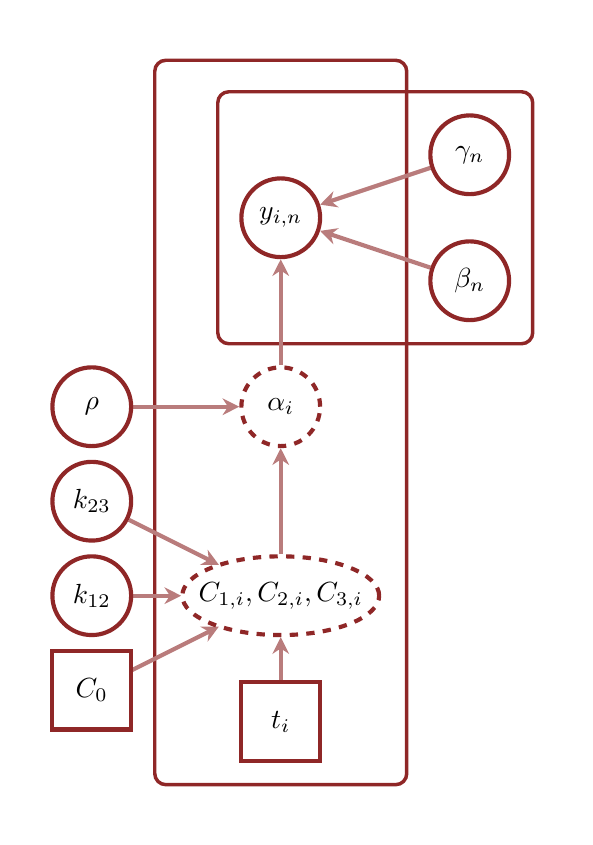
\begin{tikzpicture}[scale=0.2, thick]

  \pgfmathsetmacro{\r}{2.5}
    
  \draw[white] (-16, -6) rectangle (18, 44);

  \coordinate (A) at (0, 0);

  \coordinate (B) at (0, 8);
  
  \coordinate (C) at (-12, 2);
  \coordinate (D) at (-12, 8);
  \coordinate (E) at (-12, 14);
  
  \coordinate (F) at (0, 20);
  \coordinate (G) at (-12, 20);
  
  \coordinate (H) at (12, 28);
  \coordinate (I) at (12, 36);
  
  \coordinate (J) at (0, 32);
  
  \draw[dark, line width=1.25, rounded corners=4] (-8, -4) rectangle (8, 42);
  \draw[dark, line width=1.25, rounded corners=4] (-4, 24) rectangle (16, 40);

  \foreach \B/\E in {A/B, B/F, G/F, F/J, H/J, I/J} {
    \draw[-{Stealth[length=6pt, width=6pt]}, shorten <=15, shorten >=15, color=mid, line width=1.5] (\B) -- (\E);
  }

  \draw[-{Stealth[length=6pt, width=6pt]}, shorten <=15, shorten >=36, color=mid, line width=1.5] (D) -- (B);

  \foreach \B/\E in {C/B, E/B} {
    \draw[-{Stealth[length=6pt, width=6pt]}, shorten <=15, shorten >=25, color=mid, line width=1.5] (\B) -- (\E);
  }

  \coordinate (delta) at (\r, \r);
  \filldraw[fill=white, draw=dark, line width=1.5] ($(A) - (delta)$) rectangle ($(A) + (delta)$)
  node[color=black, midway] { $t_{i}$ };

  \filldraw[fill=white, draw=dark, dashed, line width=1.5] (B) circle [x radius=2.5 * \r, y radius=\r]
  node[color=black] { $C_{1, i}, C_{2, i}, C_{3, i}$ };

  \coordinate (delta) at (\r, \r);
  \filldraw[fill=white, draw=dark, line width=1.5] ($(C) - (delta)$) rectangle ($(C) + (delta)$)
  node[color=black, midway] { $C_{0}$ };

  \filldraw[fill=white, draw=dark, line width=1.5] (D) circle (\r)
  node[color=black] { $k_{12}$ };
  
  \filldraw[fill=white, draw=dark, line width=1.5] (E) circle (\r)
  node[color=black] { $k_{23}$ };

  \filldraw[fill=white, draw=dark, dashed, line width=1.5] (F) circle (\r)
  node[color=black] { $\alpha_{i}$ };
  
  \filldraw[fill=white, draw=dark, line width=1.5] (G) circle (\r)
  node[color=black] { $\rho$ };
  
  \filldraw[fill=white, draw=dark, line width=1.5] (H) circle (\r)
  node[color=black] { $\beta_{n}$ };
  
  \filldraw[fill=white, draw=dark, line width=1.5] (I) circle (\r)
  node[color=black] { $\gamma_{n}$ };
  
  \filldraw[fill=white, draw=dark, line width=1.5] (J) circle (\r)
  node[color=black] { $y_{i, n}$ };

\end{tikzpicture}

\end{document}  